\section{TIPE TIPE DATA GEOPASIAL}
\begin{figure}[htbp]
		\centering
		\includegraphics[width=0.75\textwidth]{pictures/gis.jpg}
		\caption{Contoh gambar GIS}
		\label{labelgambar1}
		\end{figure}	
\subsection{Pembahasan}

Data Geospasial adalah data yang memuat lokasi geografis, dimensi atau ukuran, yang mana semua nya terdapat pada permukaan bumi. Data spasial SIG mempunyai dua bagian penting yang membuatnya berbeda dari data lain, yaitu informasi lokasi dan informasi atribut. Data spasial sistem informasi geografis yang berisi informasi lokasi (informasi spasial) contohnya adalah informasi lintang dan bujur, termasuk diantaranya informasi datum dan proyeksi.

Secara umum terdapat dua metode untuk menampilkan fitur geografis kedalam GIS  atau Sistem Informasi Geospasial. Pertama, dengan struktur data vektor (vector data strukture) yang terdiri dari sebuah gambaran titik geografis, baik yang berupa tanda titik, garis, maupun poligon. Model grafik vekor ini secara terpisah fitur geografis seperti batas  administratif, jalan, bangunan, dan sungai. Sebuah objek grafis biasanya terpisah fitur geografis biasanya dikaitkan dengan informasi yang mengandung penjelasan tentang atribut objek itu, dan informasi ini bisa saja disimpan di dalam berkas spreadsheets atau pangkalan data terpisah. Kedua, dengan struktur data raster (raster data strucuture), terdiri dari serangkaian sel atau pixels yang biasa dipakai untuk menggambarkan data gambar sebagai data yang berkisinambungan. Dalam struktur data yang demikian, ada unsur resolusi sebagai ukuran dari dimensi fitur geografis yang terwakili dalam bentuk pixel. Biasanya data raster ini dipakai untuk citra satelit, ortografi digital, model elevasi digital (digital elevation models, DEM), peta digital, dan sebagainya.

Contoh lain dari informasi spasial yang bisa digunakan untuk mengidentifikasikan lokasi misalnya adalah Kode Pos. Sedangkan Informasi Atribut (deskriptif) biasa disebut juga dengan informasi non-spasial. Suatu lokalitas bisa mempunyai beberapa atribut atau properti yang berkaitan dengannya; contohnya jenis vegetasi, populasi, pendapatan per tahun, dan lain-lain.\cite{prasetyo2018estimasi}Data geospasial dibagi mejadi dua tipe jenis, diantaranya:

\begin{enumerate}
\item Data vektor adalah data yang direpresentasikan sebagai suatu mosaik berupa garis (arc/\textit{line}), polygon (daerah yang dibatasi oleh garis yang berawal dan berakhir pada titik yang sama), titik/\textit{point} (node yang mempunyai label), dan \textit{nodes} (merupakan titik perpotongan antara dua buah garis). Keuntungan utama dari format data vektor adalah ketepatan dalam merepresentasikan fitur titik, batasan dan garis lurus. Kegunaan Data Vektor untuk analisa yang membutuhkan ketepatan posisi, misalnya pada basis data batas-batas kadaster. Contoh penggunaan lainnya adalah untuk mendefinisikan hubungan spasial dari beberapa fitur. Kelemahan data vektor yang utama adalah ketidakmampuannya dalam mengakomodasi perubahan gradual. Data vektor ini disimpan dalam file ber ekstensi .shp atau shapefile esri \cite{prasetyo2018estimasi}.
	\begin{enumerate}
	\item \textit{LINE}/\textit{PATH}
	\item \textit{POLYGON}
	\item \textit{POINT}
	\end{enumerate}
		\begin{figure}[htbp]
		\centering
		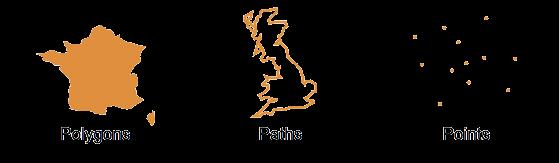
\includegraphics[width=0.75\textwidth]{pictures/datavektor.jpg}
		\caption{salah satu contoh gambar data vektor}
		\label{labelgambar2}
		\end{figure}	
	Pada gambar 1 terlihat 3 bentuk data jenis vector yaitu \textit{polygon} yang berbentuk wilayah, \textit{path} yang berbentuk garis dan point yang berbentuk titik titik.

		\begin{figure}[htbp]
		\centering
		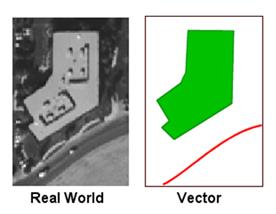
\includegraphics[width=0.65\textwidth]{pictures/olahdatavektor.jpg}
		\caption{perbandingan citra asli dengan hasil olah data vektor}
		\label{labelgambar3}
		\end{figure}
	Pada gambar 2 terlihat penerapan data \textit{vector polygon} dan \textit{ line} yang diterapkan pada salah satu bangunan. 
\item Data raster adalah data yang dihasilkan dari penginderaan jauh. Data Raster sering disebut juga dengan sel grid. Pada data raster, obyek geografis direpresentasikan sebagai struktur sel grid yang disebut dengan pixel (\textit{picture element}). Pada data raster, resolusi (definisi visual) tergantung pada ukuran pixel-nya. Dengan kata lain, resolusi pixel menggambarkan ukuran sebenarnya di permukaan bumi yang diwakili oleh setiap pixel pada citra.
Semakin kecil ukuran permukaan bumi yang direpresentasikan oleh satu sel, semakin tinggi resolusinya. Data raster sangat baik untuk merepresentasikan batas-batas yang berubah secara gradual, seperti jenis tanah, kelembaban tanah, vegetasi, suhu tanah, dan sebagainya. Kelemahan utama dari data raster adalah besarnya ukuran file; semakin tinggi resolusi grid-nya semakin besar pula ukuran filenya\cite{prasetyo2018estimasi}.
\end{enumerate}

Contoh data rester diantaranya:
\begin{enumerate}
\item Gambar citra satelit
\item Gambar PNG
\item Gambar JPG
\item Gambar Bitmap
\end{enumerate}
		\begin{figure}[htbp]
		\centering
		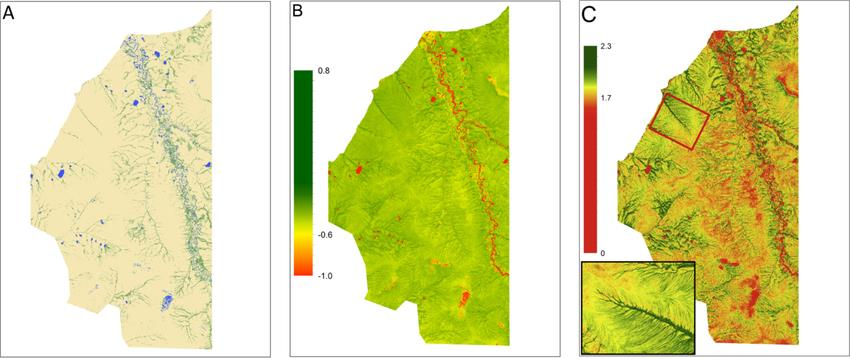
\includegraphics[width=0.65\textwidth]{pictures/dataraster.jpg}
		\caption{Gambar data raster dari tampak jauh menjadi gambar permukaan bumi seperti biasa}
		\label{labelgambar4}
		\end{figure}
Jika diliat dari penginderaan jarak jauh, maka data raster ini seperti gambar permukaan bumi pada biasanya, namun jika di \textit{zoom} lebih dekat maka akan muncul terlihat \textit{pixel pixel} nya.
		\begin{figure}[htbp]
		\centering
		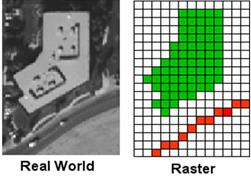
\includegraphics[width=0.65\textwidth]{pictures/datarasterzoom.jpg}
		\caption{Data raster jika di \textit{zoom} ke ukuran aslinya maka nampak \textit{pixel pixel} nya}
		\label{labelgambar5}
		\end{figure}
Pada gambar 4 terlihat penerapan data raster pada salah satu bangunan yang hasilnya berbentuk \textit{pixel pixel} gambar. \textit{Pixel} gambar tersebut muncul karna gambar telah di \textit{zoom} atau dalam bentuk resolusi yang kecil.

Berikut ditampilkan perbedaan nampak dari kedua data yang telah dipaparkan
		\begin{figure}[htbp]
		\centering
		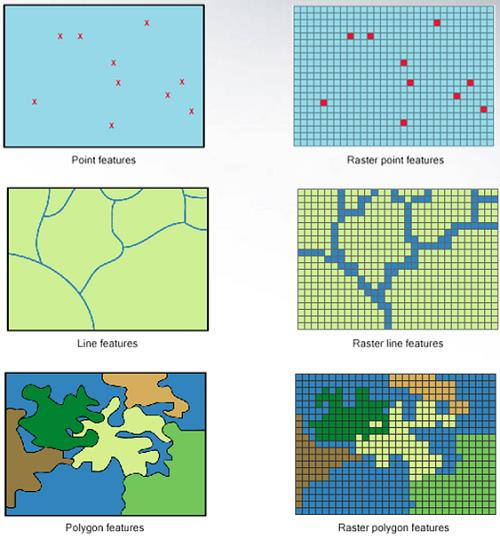
\includegraphics[width=0.65\textwidth]{pictures/perbedaan.jpg}
		\caption{Perbedaan data \textit{raster} dan \textit{vektor} pada 3 jenis penerapan.}
		\label{labelgambar6}
		\end{figure}
\section{Srukture Data GIS}
Data geografi meliputi informasi tentang posisi, hubungan topologi dan aspek spasial dari pemrosesan data. Data ini menggambarkan obyek dan fenomena geografinya. Obyek mengacu pada lokasinya pada permukaan bumi dengan menggunakan sistem koordinat 9dapat berupa lokal, nasional, maupun internasional). Sedangkan fenomena geografi dapat berupa konsep fenomenologi, sepertikota, sungai, dataran rendah/tinggi, bentuk serta struktur tanah, dan sebagainya. Fenomena geografi ini akan membawa ke dalam bentuk blok klasifikasi atau taksonomi secara hirarkis, seperti negara-propinsi-kabupaten-kecamatan-kelurahan, klasifikasi bentuk struktur tanah,vegetasi, dan sebagainya.Semua data geografi dapat disajikan dalam tiga bentuk dasar konsep topologi, yaitu:
\begin{enumerate}
\item Titik (point)
\item Garis (line)
\item Luasan(area)
\end{enumerate}
Setiap fenomena geografi pada dasarnya dapat disajikan ke dalam tiga bentuk dasar di atas, disertai dengan label yang menerangkan apa disajikan tersebut. Dalam aktivitas penelitian, perencanaan, atau pengambilan keputusan diperlukan data dan informasi yang baik dan teratur agar pekerjaan yang dilakukan dengan cepat dan tepat dapat diselesaikan. Pengaturan dan pengumpulan data secara manual biasa dilakukan berdasarkan hirarki topologi. Peta yang memuat berbagai macam data dan informasi, menyimpan data dalam bentuk topologi. Data keruangan dalam terminologi fisikal dan lokasi geografi. Bentuk data yang dapat dijadikan masukan kedalam notasi yang menunjukkan lokasi keruangan adalah titik, garis, dan area atau poligon. Semua data dari kenampakan, dan fenomena geografi dapat digambarkan melalui salah satu bentuk notasi tersebut.
\subsection{Cara Kerja Gis}
 GIS dapat mempersentasikan suatu model “real world” (dunia nyata) di atas layer monitor komputer sebagaimana lembaran-lembaran peta dapat mempresentasikan dunia nyata di atas kertas. Walaupun demikian, GIS memiliki kekuatan lebih dan daya flesksibelitas dari pada lembaran-lembaran peta kertas. Peta merupakan salah satu bentuk reperesentasi grafis miliki dunia nyata objekobjek yang direpresentasikan di atas peta disebut sebagai unsur-unsur peta atau map feature (sebagai contoh adalah sungai, jalan, gunung, bangunan, dan lainlain) karena peta mengorganisasikan unsur-unsurnya berdasarkan lokasi masingmasin, maka peta sangat baik di dalam memperlihatkan hubungan atau relasi yang dimiliki oleh unsur-unsurnya. Sebagai ilustrasi, berikut adalah contoh-contoh hubungan tersebut :
\begin{enumerate}
\item Suatu gedung terletak di dalam wilayah kecamatan tertentu.
\item Jembatan melintas di atas suatu sungai.
\item Bangunan kuno bersebelahan dengan taman.
\end{enumerate}
Berikut merupakan contoh peta kota bandung seperti pada gambar \ref{kotapetabandung}
\begin{figure}[ht]
	\centerline{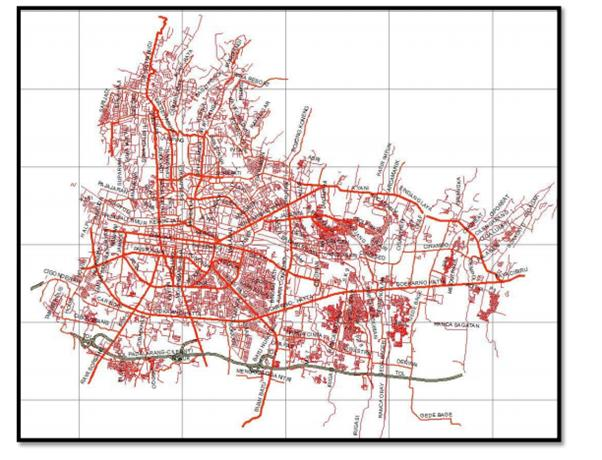
\includegraphics[width=0.60\textwidth]{pictures/bnd.jpg}}
	\caption{contoh peta kota bandung}
	\label{kotapetabandung}
	\end{figure}

\section{PENGENALAN TENTANG LONGITUDE,LATITUDE,BUJUR,DAN LINTANG}
\subsection{Sistem Koordinat}
Sistem koordinat dimaksudkan untuk memberikan peng-alamat-an terhadap setiap lokasi di permukaan bumi. Peng-alamat-an dengan sistem koordinat didasarkan atas jarak timur-barat dan utara-selatan suatu tempat dari suatu \textit{titik pangkal} tertentu. Jarak diukur dalam satuan derajat sudut yang dibentuk dari titik pangkal ke posisi tersebut yang melalui pusat bumi. Sedangkan titik pangkal ditetapkan berada di perpotongan belahan utara-selatan bumi (garis khatulistiwa) dengan garis yang membelah bumi timur-barat melalui kota Greenwich di Inggris. berikut adalah contoh gambar sistem kordinat dengan globe \ref{kordinat}
\begin{figure}[ht]
	\centerline{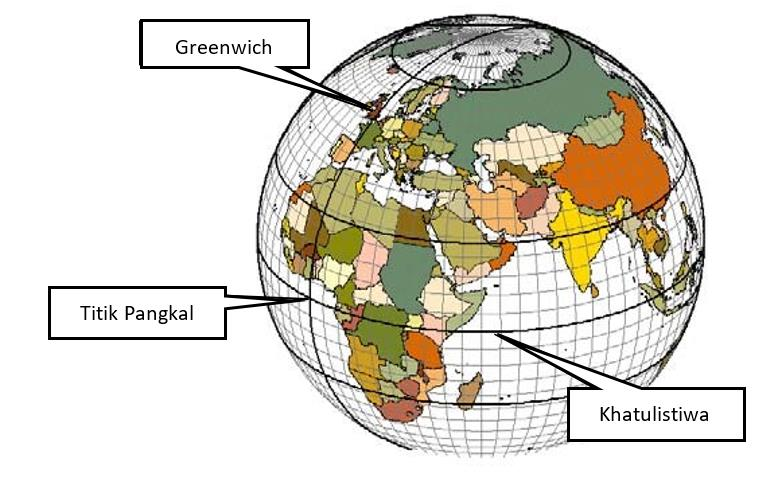
\includegraphics[width=0.70\textwidth]{pictures/kordinat.jpg}}
	\caption{contoh sitem koordinat dengan globe}
	\label{kordinat}
	\end{figure}

Posisi suatu tempat di-alamatkan dengan nilai koordinat garis bujur (longitude) dan lintang (latitude) yang melalui tempat itu. Garis bujur (longitude), sering juga disebut meridian, yaitu merupakan garis lurus yang menghubungkan kutub utara dan selatan bumi. Nilai koordinat garis bujur dimulai dari bujur 0 (drajat) yaitu di Greenwich, kemudian membesar ke arah timur dan barat sampai bertemu kembali di Garis batas tanggal internasional yaitu terletak di Selat Bering dengan nilai 180 (drajat). Garis bujur 0(drajat) sering sekali disebut prime meridian atau meridian Greenwich. Garis bujur ke arah barat diberi nilai negatif dan disebut dengan bujur barat (west longitude) serta disingkat BB. Sedangkan garis bujur yang ke arah timur diberi nilai positif dan disebut dengan bujur timur (east longitude) disingkat BT. Nilai koordinatnya didasarkan atas besarnya sudut yang terbentuk dari bujur 0 ke garis bujur tersebut melalui pusat bumi.

Untuk nilai koordinat lintang dimulai dari garis lingkaran katulistiwa yang diberi nilai 0(drajat). Selanjutnya garis lintang yang lain berupa lingkaran-lingkaran paralel (sejajar) khatulistiwa berada di sebelah utara dan selatan khatulistiwa. Lingkaran paralel di selatan disebut dengan garis lintang selatan (LS) dan diberi nilai negatif, sedangkan lingkaran paralel di utara diberi nilai positif  dan disebut garis lintang utara (LU). Nilai maksimum untuk koordinat garis lintang adalah 90(drajat) yaitu terletak di kutub-kutub bumi.

Lingkaran paralel yang merupakan representasi dari garis lintang ini semakin mengecil ukurannya dengan semakin jauh dari khatulistiwa. Sehingga jarak 1o timur-barat di khatulistiwa jauh lebih besar daripada jarak 1(derajat) timur-barat di tempat yang jauh dari khatulistiwa. Di khatulistiwa 1(derajat) timur-barat sama dengan 111,321 Km, tetapi di dekat kutub 1(derajat) timur-barat hanya beberapa meter saja. Itu sebabnya grid yang dibuat dari garis lintang dan garis bujur tampak berupa bujur sangkar di khatulistiwa dan berupa persegi panjang di daerah dekat kutub. Koordinat yaitu bilangan yang dipakai untuk menunjukkan lokasi suatu titik di garis permukaan atau ruang. Koordinat dapat memudahkan kita dalam menemukan letak suatu benda.
\subsection{Macam-macam Sistem Koordinat}
Adapun beberapa macam sistem koordinat, antara lain:
\begin{enumerate}
\item Sistem Koordinat Kartesius
Untuk menyatakan posisi sebuah benda dibutuhkan suatu sistem koordinat yang memiliki pusat koordinat dan sumbu koordinat. Sistem koordinat yang paling dasar/sederhana adalah sistem koordinat kartesius. Jika berbicara ruang dua dimensi, maka koordinat kartesius dua dimensi memiliki pusat di O dan dua sumbu koordinat yang saling tegak lurus yaitu x dan y. Dalam gambar dibawah in \ref{kartesius}, titik P dinyatakan dalam koordinat x dan y.
\begin{figure}[ht]
	\centerline{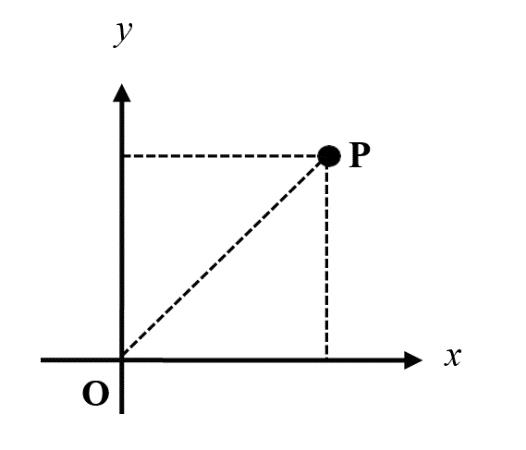
\includegraphics[width=0.65\textwidth]{pictures/kordinatkartesius.jpg}}
	\caption{Sistem kordinat kartesius}
	\label{kartesius}
	\end{figure}
Bulan dalam berevolusi mengelilingi bumi, suatu saat bulan berada pada arah yang berlawanan dengan matahari dan posisi matahari, bumi dan bulan berada pada suatu garis lurus yang disebut bulan purnama (\textit {full moon}). Bulan purnama juga sering disebut dengan istilah istiqbal. (Azhari, 2007:19).

Gambar \ref{kartesius}. dapat digunakan untuk menentukan waktu terjadinya bulan purnama. Waktu bulan purnama dapat dicari melalui titik potong antara lintasan edar matahari dan bulan yang saling berpotongan. Jika posisi matahari dan bulan pada saat bulan purnama berada pada titik potong tersebut, maka rumus persamaan garis lurus dapat digunakan untuk menentukan waktu terjadinya bulan purnama. Garis lurus adalah sebuah garis yang merupakan objek geometris, jika ditempatkan pada suatu bidang koordinat maka garis ini akan mempunyai  persamaan yaitu persamaan garis lurus. Persamaan garis lurus adalah suatu persamaan yang jika digambarkan ke dalam bidang koordinat kartesius akan membentuk sebuah garis lurus. Untuk mengetahui persamaan garis lurus, maka diperlukan suatu kemiringan garis (gradien).
	\begin{enumerate}
	\item Gradien
	\end{enumerate}
\end{enumerate}